\documentclass[a4paper,12pt]{article}
\usepackage{standalone}
\usepackage{amsmath}
\usepackage{amssymb}
\usepackage{graphicx}
\usepackage{caption}
\usepackage{subcaption}
\usepackage[parfill]{parskip}
\usepackage{xcolor}
\usepackage{array}
\usepackage{xfrac}
\usepackage{wrapfig}
\usepackage{xcolor}
\usepackage{enumitem}
\usepackage[backend=biber, bibencoding=utf8, url=false, doi=false, isbn=false, maxbibnames=2, giveninits=true]{biblatex}
\usepackage[margin=0.5in]{geometry}

\usepackage{verbatim}

% Tikz/pgf
\usepackage{pgfplots}
\usepackage{pgfplotstable}
\pgfplotsset{compat=1.16}

\DeclareUnicodeCharacter{0301}{\'{e}}
% Removes "In: " in 
\renewbibmacro{in:}{}
\DeclareSourcemap{%
  \maps[datatype=bibtex]{
    \map{
      \step[fieldsource=journaltitle, match={Physica D: Nonlinear Phenomena},
      replace={Physica D}]%
    }
  }
}
\DeclareSourcemap{%
  \maps[datatype=bibtex]{
   \map{
      \step[fieldsource=journaltitle, match={Physical Review E},
      replace={Phys Rev E}]%
    }
  }
}
\DeclareSourcemap{%
  \maps[datatype=bibtex]{
   \map{
      \step[fieldsource=journaltitle, match={Chaos: An Interdisciplinary Journal of Nonlinear Science},
      replace={Chaos}]%
    }
  }
}
\DeclareSourcemap{%
   \maps[datatype=bibtex]{
     \map{
         \step[fieldsource=journaltitle, match={Journal of Physics A: Mathe    matical and General},
         replace={J Phys A-Math Gen}]%
     }
   }
}

% COMMANDS
% s = seq(n, m, length=k) = n + (m - n)/(k - 1) * i, i = 0,\dots,k-1
\newcommand{\identf}{\mathcal{I}}
\newcommand{\SD}{ \left\lbrace \alpha_1^c, \alpha_3^c, \alpha_2^s, \alpha_3^s \right\rbrace }
\newcommand{\ND}{ \left\lbrace \alpha_0^c, \alpha_2^c, \alpha_0^s, \alpha_1^s \right\rbrace }
\newcommand{\dyval}[3]{#1 + \dfrac{#2 - #1}{#3 - 1} * i}
\newcommand{\EQ}[1]{Eq. \eqref{#1}}

\newcommand{\di}{d^I}
\newcommand{\dc}{d^C}
\newcommand{\ds}{d^F}
\newcommand{\deff}{D_\text{eff}}
\newcommand{\MFPT}{\langle t(\mathcal{L} - x(0)) \rangle}

% PATH TO IMAGES
% \graphicspath{{./PathONE/}{./PathTWO/}
\graphicspath{{./images/}}

% BIBLIOGRAPHY ITEM (e.g. NAME OF ZOTERO FOLDER)
\addbibresource{~/Dropbox/ZotLibrary.bib}



\begin{document}
\tableofcontents
Notations:
\begin{itemize}
    \item $\alpha$ - Internal angle of parallel channel
    \item $d$ - Pore width
    \item $M$ - Number of intial conditions (random position and uniform velocity unless stated otherwise)
    \item $T$ - Total time (length of all billiard paths)
    \item $N$ - Number of collisions
    \item $\mu(t; z) = \dfrac{\log \langle \Delta x^2(t) \rangle - \log \langle \Delta x^2 (t^z) \rangle}{(1 - z) \log t}$ - Power scaling
    \item $\tau_j$ - First passage time of $j$th particle
\end{itemize}



\clearpage
\subsubsection{First passage time distribution}

%\begin{figure}
%    \centering
%    \begin{tikzpicture}
%    \begin{axis}[
%             xlabel={$t$},
%             ylabel={$S(t$},
%             xmode=log, 
%             ymode=log,
%             legend pos=south west,
%             grid=both, grid style={line width=.1pt, draw=black!10}, major grid style={line width=.2pt,draw=black!50},
%             minor tick num=5,
%             % xmin=,
%             % xmax=,
%             ymin=0.01,
%             ymax=1,
%            ]
%        % \addplot+[const plot, no marks, thin, red]     table[x index={0}, y index={1}, unbounded coords=jump,] {T4/ECDF.pgf};
%            \addplot {x};
%    \end{axis}
%    \end{tikzpicture}
%    \caption{With  . }
%    \label{fig:}
%\end{figure}

\clearpage
\subsubsection{First passage time density}

\clearpage
\subsubsection{Mean first passage time}

%\begin{figure}
%    \centering
%    \begin{tikzpicture}
%    \begin{axis}[
%             ylabel={$\langle \tau(L) \rangle$},
%             xlabel={$L$},
%             xmode=log, 
%             ymode=log,
%             legend pos=south west,
%             grid=both, grid style={line width=.1pt, draw=black!10}, major grid style={line width=.2pt,draw=black!50},
%             minor tick num=5,
%             % xmin=,
%             % xmax=,
%             ymin=0.01,
%             ymax=1,
%            ]
%        % \addplot+[const plot, no marks, thin, red]     table[x index={0}, y index={1}, unbounded coords=jump,] {T4/ECDF.pgf};
%        %\addplot table[x index={0}, y index=] {../Data/EscapeToAbsorbingBoundary/1-0-MFPT.dat};
%            \addplot {x};
%    \end{axis}
%    \end{tikzpicture}
%    \caption{With  . }
%    \label{fig:}
%\end{figure}


\clearpage
\subsubsection{First passage time as function of initial conditions}

\clearpage
\subsubsection{Escape to a symbolic sequence}
Denote the four walls of a parallel channel with the symbols $\{ 0,1,3,4 \}$ taken in order of increasing arc length, starting at $(0, 0)$ and ending at $(0, d)$. We record the first passage time as the time at which a particular sequence is first observed.


\begin{figure}
    \centering
    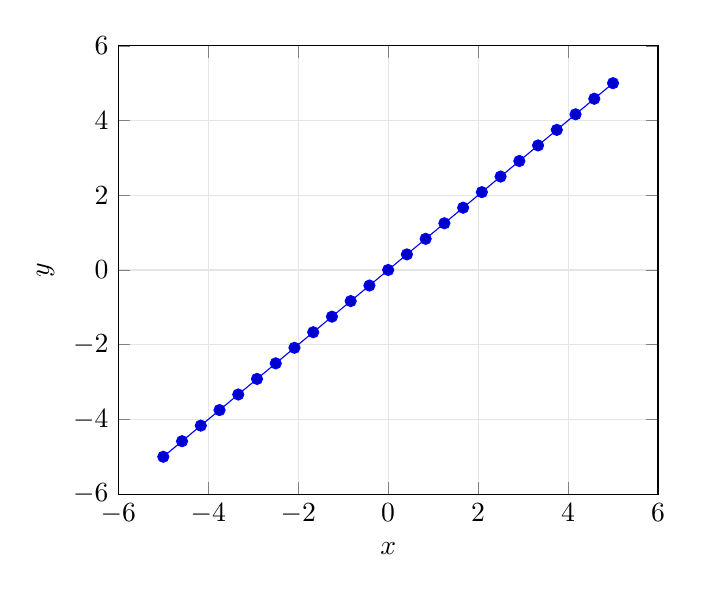
\begin{tikzpicture}
    \begin{axis}[
            xlabel={$x$},
            ylabel={$y$},
            grid=both, grid style={draw=black!10},
            %xmin=, 
            %xmax=,
            %ymin=,
            %ymax=,
            %legend pos=,
        ]
    
       \addplot {x};
       %\foreach \i in {5,...,8} {
       %     \addplot+[] table[x index={0}, y index={\i}] {Data.pgf}; 
       %     \pgfmathparse{int(\i - 5)}
       %     \addlegendentryexpanded{$\alpha_{\pgfmathresult}^s$}
       %}
    
    \end{axis}
    \end{tikzpicture}
\caption{this}
\end{figure}



%\begin{figure}[!ht]
%    \centering
%    \includegraphics[width=\textwidth]{ResultListFigures/FPTSymb.pdf}
%    \caption{Shown are the empirical distributions of first passage times defined by escapes to a bouncing ball symbolic sequence of increasing length. Sequences are ``040404040" (black), ``04040404040" (red), ``0404040404040" (green) and ``040404040404040" (blue). A value of $\infty$ is assigned to those particles which never escape to the chosen sequence within $10^4$ collisions.
% }
%    \label{fig:}
%\end{figure}
%
%\clearpage
%\subsubsection{Escape to a randomly selected collision number}
%For $M$ trajectories containing $N$ collisions, we select a uniformly distributed collison number and take the total time at that collision as the first passage time. The survival probability is then a linear function.
%\begin{figure}[!ht]
%    \centering
%    \includegraphics[width=\textwidth]{ResultListFigures/FPTRandom.pdf}
%    \caption{Survival probability for particles escaping to a uniformly distributed collision number $\sim [1, 10^5]$.}
%    \label{fig:}
%\end{figure}

%\clearpage
%\subsubsection{Trajectory length distributions}
%\begin{figure}[!ht]
%    \centering
%    \includegraphics[width=\textwidth]{ResultListFigures/TimeAtCollisions.pdf}
%    \caption{Distributions of trajectory lengths after some number of collisions.}
%    \label{fig:}
%\end{figure}


%\clearpage
%\subsubsection{Mean time at collision}
%\begin{figure}[!ht]
%    \centering
%    \includegraphics[width=\textwidth]{ResultListFigures/TimeAtCollisions.pdf}
%    \caption{The length of a trajectory for collision numbers $n \in [1, N]$ is typically linear. The slope of }
%    \label{fig:}
%\end{figure}
%
%
%
%\subsubsection{Spatially averaged times}
%
%For trajectories of length $T$, we consider the distribution of times within  
%
%\clearpage
%\subsubsection{Distribution of unidirectional escapes}
%Given the indicator function,
%\begin{equation}
%    \xi(x) = 
%    \begin{cases} 
%        +1  & \text{if} \ x > 0 \\
%        -1 & \text{if} \ x < 0
%    \end{cases}
%\end{equation}
%we consider distribution of counts
%\begin{equation}
%    C_j = \sum_{i = 0}^K \xi(x_j^i(\tau_j))
%\end{equation}
%where $x_j^i(\tau_j) = \pm L_i$ is the resting $x$-position of the $j$th particle escaping from absorbing boundaries located at $\pm L_i$. Thus $|C_j| = L_K$ corresponds to a particle which escaped exlusively from the left or right sides of the channel. This situation tends to be the case for about half of the particles. Looking only at particles which escape from at least two sides of the channel, we find the following histogram.
%\begin{figure}[!ht]
%    \centering
%    \includegraphics[width=\textwidth]{ResultListFigures/NetLREscapesPerParticle.pdf}
%    \caption{Distribution of the $C_j$'s defined above. Shown only are particles which escapein at least one positive and negative directions.}
%    \label{fig:}
%\end{figure}
%
%
%
%\clearpage
%\subsubsection{Number of left/right escapers}
%\begin{figure}[!ht]
%    \centering
%    \includegraphics[width=\textwidth]{ResultListFigures/NetLREscapes.pdf}
%    \caption{Net number of left/right escapes for each $L$ (shown on the vertical axis) is given by $\sum_{j=1}^{M} \xi(x_j^i(\tau_j))$ where $\xi$ is the indicator function from the previous section. Results from four independant simulations are shown, each involving $10^5$ particles.}
%    \label{fig:}
%\end{figure}
%


\subsubsection{Escape direction distribution}
Consider the distribution of particle directions $\theta_j(\tau_j)$.


\subsubsection{First passage time distribution within finite time}
Unlike before, we consider only those particles which \emph{do} escape within our chosen total time $T$. This is achieved through rejection sampling. For $L = 10,20,\dots,100$, consider $T = 10^3, 10^4, \dots, 10^6$ such that $M = 10^4$ particles escape within those times. We find the vast majority of particles to 





\cleardoublepage
\subsection*{References}
\printbibliography[heading=none] % See options here: https://www.overleaf.com/learn/latex/Bibliography_management_with_biblatex

%\dfrac{5 \pi }{10 + 25 \varphi } + \dfrac{\dfrac{5 \pi}{2 + 5 \varphi} -\dfrac{5 \pi }{10 + 25 \varphi } }{8} i \ i = 
\end{document}


